% Chapter Template

\chapter{Praxis} % Main chapter title

\label{Chapter5} % Change X to a consecutive number; for referencing this chapter elsewhere, use \ref{ChapterX}

\lhead{Chapter 5. \emph{Ergebnisse}} % Change X to a consecutive number; this is for the header on each page - perhaps a shortened title

%----------------------------------------------------------------------------------------
%	PRAXIS
%----------------------------------------------------------------------------------------

\section{Implementierung}


%
% AUFBAU
%
\subsection{Aufbau mein Programm}

\begin{figure}[ht]
	\centering
  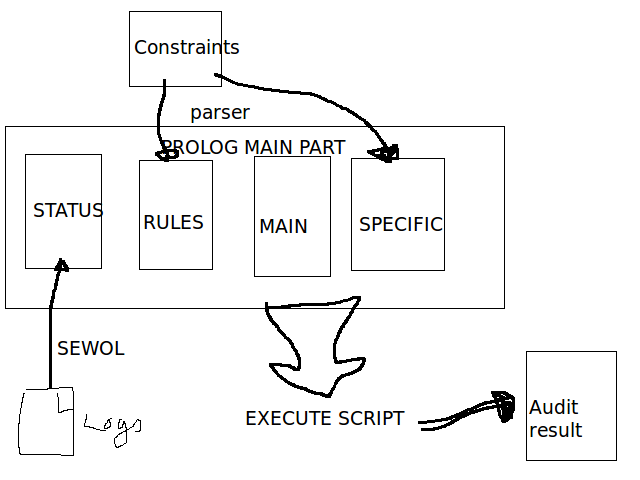
\includegraphics[width=0.9\textwidth]{Figures/myProg}
	\caption{Aufbau mein Programm}
	\label{fig: myprog}
\end{figure}

Das Programm liest mittels SEWOL MXML logs ein und übersetzt sie in Status Prädikate. 
Die Constraints werden ebenfalls eingelesen und in Regelprädikate übersetzt. Der Parser für die Grammatik wurde mit ANTLR\cite{antlr} erzeugt.
Die eigentliche Untersuchung kann entweder durch ein Skript oder innerhalb des Javacodes gestartet werden.

\subsection{Wissensbasis}
Die Wissensbasis wird aus den Logs herausgelesen und in entsprechende Prädikate übersetzt. Auf Basis dieser Prädikate arbeitet der Modelchecker. Die Wissensbasis besteht aus genau 7 möglichen Prädikaten, welche ausreichen, um die Events vollständig wiederzugeben:\\

\begin{enumerate}
\item \textbf{workflow{\_}name(caseID, workflowName)}: Weist einer Case ID einen eindeutigen Namen hinzu, welcher der Workflow Spezifikation entspricht. Die Case ID kennzeichnet die Instanz, konkrete Ausführung eines Workflows. Dieses Prädikat dient jedoch nur zur Vollständigkeit. Sollte es für den Arbeitsablauf keinen eindeutigen Namen geben, wird dieses Prädikat nicht gesetzt. Es kann im Modelchecker dann auch nicht darauf zugegriffen werden.
\item \textbf{activity{\_}workflow(activityID, caseID)}: Setzt fest, zu welcher case ID die Activity gehört. TaskID wird intern vom Transformer gesetzt.
\item \textbf{activity{\_}name(taskID, taskName)}: Legt den Namen der Activity fest. Dieser ist im MXML Modell als WorkflowModelElement zu finden.
\item \textbf{timestamp(taskID, timestamp in ms)}: Zeitpunkt der Aktivität in ms nach 1970. Sollte kein Zeitpunkt eingetragen sein, wird entweder kein Fakt gesetzt, oder es wird die Reihenfolge der Einträge genommen. Dazu wird der letzte Wert + 1 ms gesetzt.
\item \textbf{eventtype(taskID, eventtype)}: Der Eventtyp der Aktivität. Im Grundmodell sind es start, accept, abort, ... Kann jedoch varriieren.
\item \textbf{executed{\_}user(user, taskID)}: Der Nutzer, der die Activity ausgeführt hat.
\item \textbf{executed{\_}group(group, taskID)}: Die Rolle, in der die Activity ausgeführt wurde. Man beachte, dass ein Nutzer mehrere Rollen haben kann.
\item \textbf{task{\_}attribute(taskID, attrName, attrType, attrValue)}: In dieser Wissensbasis wird zwischen zwei Typen unterschieden. String-Attributen, welche nur Vergleichsoperatoren kennen. Hat das Attribut im ürsprünglichen Event ein anderes Format, muss es für die Analyse in eine passende String Darstellung konvertiert werden. 
\end{enumerate}

Die erste Zeile aus dem Eventlog aus Tabelle \ref{tab:examplelog} wird in folgende Wissensbasis konvertiert:
\begin{table}[h]
\begin{tabular}{ccc}
activity{\_}workflow(0,0) & activity{\_}name(0,'Approach check') & timestamp(0, 123)\\ 
eventtype(0, start) & executed{\_}user(0, 'Mark') & executed{\_}role(0, 'Admin') 
\end{tabular}
\caption{fd}
\label{tab:knowledge}
\end{table}



TODO: Closed World, was passiert mit nicht angegebenen Zeiten,.

%
% EINGABE DER REGELN
%
\subsection{Übersetzung der Regeln}
Die Regeln werden in einer oder mehreren Dateien definiert und von dem ConstraintReader zuerst in speziellen Containern gespeichert, dort sortiert und angepasst und anschließend in zwei Prologdateien geschrieben, die später vom eigentlichen modelchecker verwendet werden.

\begin{figure}[ht]
	\centering
  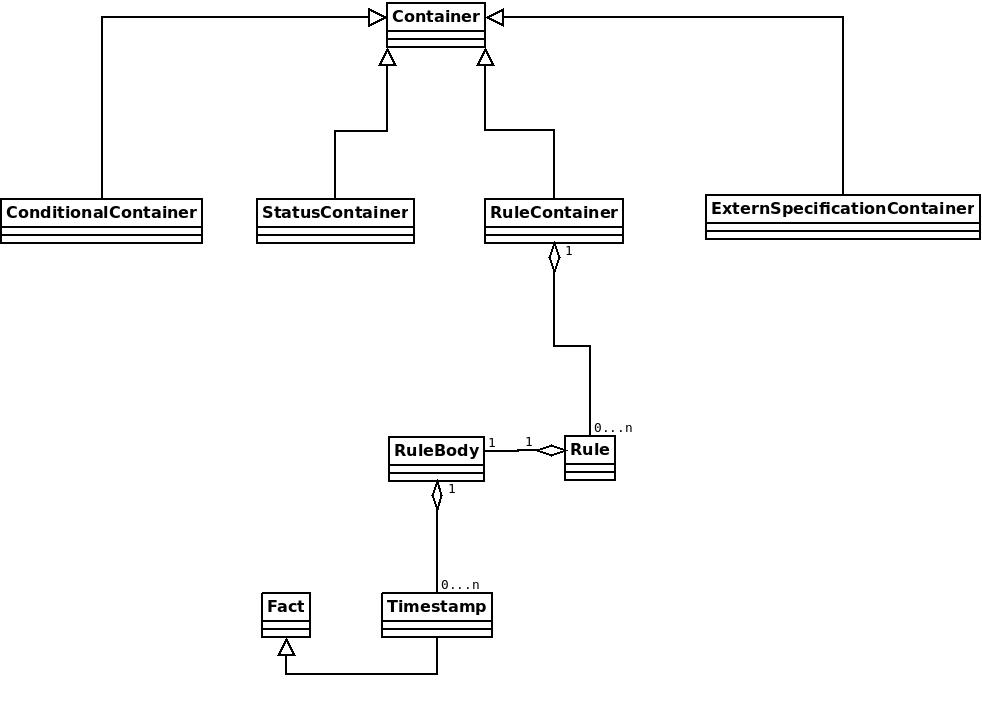
\includegraphics[width=0.9\textwidth]{Figures/Container}
	\caption{Interne Datenstruktur}
	\label{fig:container}
\end{figure}

%
% ALGORITHMUS
%
\subsection{Algorithmus Modelchecker}


\begin{verbatim}
3. Add Collaborators
4. Adddominates
   Addrelated
5. For each cannot_execute_user(Actor, Activity): 
6.	If exists executed_user(Actor, Activity) 
7. 	then write trace
8. For each cannot_execute_role(Role, Activity):
9. 	If exists executed_role(Role, Activity)
10.	then write trace
11. For each must_execute_user(Actor, Activity): 
12.	If not exists executed_user(Actor, Activity) 
13. 	then write trace
14. For each must_execute_role(Role, Activity):
15. 	If not exists executed_role(Role, Activity)
16.	then write trace
17. For each panic write trace
\end{verbatim}
\begin{figure}[!h]
\caption{Pseudocode des Modelchecker}
\label{fig:pseudocode}
\end{figure}

Zuerst aus Logs Status-Prädikate auslesen.\\
Für jedes critical task pair entsprechende collaborateurs setzen.\\
Schleife über Regeln\\
--Die resultierenden Heads bestimmen und schauen, ob es für cannot do ein executed und für must do kein executed gibt-> dann wurde es verletzt. Um das herauszufinden, wird die Regel in executed $ - >$ blabla, oder not(executed) $- >$ blabla übersetzt.\\
 
Einfaches Beispiel: Rule: executed(ui, t1)-> cannot do(ui,t2) und status: executed('tom', t1). Daraus wird abgeleitet: cannot do('tom', t2). Da es nicht in der DB ist, ist alles OK
